\FChapter{Chapter Thirty-Six}{36}

\Lettrine{T}{he} \textsc{daylight came.} I rose at dawn. I busied myself for an hour or two
with arranging my things in my chamber, drawers, and wardrobe, in the
order wherein I should wish to leave them during a brief absence. 
Meantime, I heard \St{} John quit his room. He stopped at my door: I
feared he would knock---no, but a slip of paper was passed under the
door. I took it up. It bore these words---

\enquote{You left me too suddenly last night. Had you stayed but a little
longer, you would have laid your hand on the Christian's cross and the
angel's crown. I shall expect your clear decision when I return this
day fortnight. Meantime, watch and pray that you enter not into
temptation: the spirit, I trust, is willing, but the flesh, I see, is
weak. I shall pray for you hourly.---Yours, {\St{} John}.}

\enquote{My spirit,} I answered mentally, \enquote{is willing to do what
is right; and my flesh, I hope, is strong enough to accomplish the will
of Heaven, when once that will is distinctly known to me. At any rate,
it shall be strong enough to search---inquire---to grope an outlet from
this cloud of doubt, and find the open day of certainty.}

It was the first of June; yet the morning was overcast and chilly: rain
beat fast on my casement. I heard the front-door open, and \St{} John
pass out. Looking through the window, I saw him traverse the garden. 
He took the way over the misty moors in the direction of
Whitcross---there he would meet the coach.

\enquote{In a few more hours I shall succeed you in that track, cousin,}
thought I: \enquote{I too have a coach to meet at Whitcross. I too have
some to see and ask after in England, before I depart for ever.}

It wanted yet two hours of breakfast-time. I filled the interval in
walking softly about my room, and pondering the visitation which had
given my plans their present bent. I recalled that inward sensation I
had experienced: for I could recall it, with all its unspeakable
strangeness. I recalled the voice I had heard; again I questioned
whence it came, as vainly as before: it seemed in \emph{me}---not in the
external world. I asked was it a mere nervous impression---a delusion? 
I could not conceive or believe: it was more like an inspiration. The
wondrous shock of feeling had come like the earthquake which shook the
foundations of Paul and Silas's prison; it had opened the doors of the
soul's cell and loosed its bands---it had wakened it out of its sleep,
whence it sprang trembling, listening, aghast; then vibrated thrice a
cry on my startled ear, and in my quaking heart and through my spirit,
which neither feared nor shook, but exulted as if in joy over the
success of one effort it had been privileged to make, independent of the
cumbrous body.

\enquote{Ere many days,} I said, as I terminated my musings, \enquote{I
will know something of him whose voice seemed last night to summon me. 
Letters have proved of no avail---personal inquiry shall replace them.}

At breakfast I announced to Diana and Mary that I was going a journey,
and should be absent at least four days.

\enquote{Alone, Jane?} they asked.

\enquote{Yes; it was to see or hear news of a friend about whom I had
for some time been uneasy.}

They might have said, as I have no doubt they thought, that they had
believed me to be without any friends save them: for, indeed, I had
often said so; but, with their true natural delicacy, they abstained
from comment, except that Diana asked me if I was sure I was well enough
to travel. I looked very pale, she observed. I replied, that nothing
ailed me save anxiety of mind, which I hoped soon to alleviate.

It was easy to make my further arrangements; for I was troubled with no
inquiries---no surmises. Having once explained to them that I could not
now be explicit about my plans, they kindly and wisely acquiesced in the
silence with which I pursued them, according to me the privilege of free
action I should under similar circumstances have accorded them.

I left Moor House at three o'clock \PM, and soon after four I stood at
the foot of the sign-post of Whitcross, waiting the arrival of the coach
which was to take me to distant Thornfield. Amidst the silence of those
solitary roads and desert hills, I heard it approach from a great
distance. It was the same vehicle whence, a year ago, I had alighted
one summer evening on this very spot---how desolate, and hopeless, and
objectless! It stopped as I beckoned. I entered---not now obliged to
part with my whole fortune as the price of its accommodation. Once more
on the road to Thornfield, I felt like the messenger-pigeon flying home.

It was a journey of six-and-thirty hours. I had set out from Whitcross
on a Tuesday afternoon, and early on the succeeding Thursday morning the
coach stopped to water the horses at a wayside inn, situated in the
midst of scenery whose green hedges and large fields and low pastoral
hills (how mild of feature and verdant of hue compared with the stern
North-Midland moors of Morton!) met my eye like the lineaments of a once
familiar face. Yes, I knew the character of this landscape: I was sure
we were near my bourne.

\enquote{How far is Thornfield Hall from here?} I asked of the ostler.

\enquote{Just two miles, ma'am, across the fields.}

\enquote{My journey is closed,} I thought to myself. I got out of the
coach, gave a box I had into the ostler's charge, to be kept till I
called for it; paid my fare; satisfied the coachman, and was going: the
brightening day gleamed on the sign of the inn, and I read in gilt
letters, \enquote{The Rochester Arms.} My heart leapt up: I was already
on my master's very lands. It fell again: the thought struck it:---

\enquote{Your master himself may be beyond the British Channel, for
aught you know: and then, if he is at Thornfield Hall, towards which you
hasten, who besides him is there? His lunatic wife: and you have
nothing to do with him: you dare not speak to him or seek his presence. 
You have lost your labour---you had better go no farther,} urged the
monitor. \enquote{Ask information of the people at the inn; they can
give you all you seek: they can solve your doubts at once. Go up to
that man, and inquire if \Mr{} Rochester be at home.}

The suggestion was sensible, and yet I could not force myself to act on
it. I so dreaded a reply that would crush me with despair. To prolong
doubt was to prolong hope. I might yet once more see the Hall under the
ray of her star. There was the stile before me---the very fields
through which I had hurried, blind, deaf, distracted with a revengeful
fury tracking and scourging me, on the morning I fled from Thornfield:
ere I well knew what course I had resolved to take, I was in the midst
of them. How fast I walked! How I ran sometimes! How I looked forward
to catch the first view of the well-known woods! With what feelings I
welcomed single trees I knew, and familiar glimpses of meadow and hill
between them!

At last the woods rose; the rookery clustered dark; a loud cawing broke
the morning stillness. Strange delight inspired me: on I hastened. 
Another field crossed---a lane threaded---and there were the courtyard
walls---the back offices: the house itself, the rookery still hid. 
\enquote{My first view of it shall be in front,} I determined,
\enquote{where its bold battlements will strike the eye nobly at once,
and where I can single out my master's very window: perhaps he will be
standing at it---he rises early: perhaps he is now walking in the
orchard, or on the pavement in front. Could I but see him!---but a
moment! Surely, in that case, I should not be so mad as to run to him? 
I cannot tell---I am not certain. And if I did---what then? God bless
him! What then? Who would be hurt by my once more tasting the life his
glance can give me? I rave: perhaps at this moment he is watching the
sun rise over the Pyrenees, or on the tideless sea of the south.}

I had coasted along the lower wall of the orchard---turned its angle:
there was a gate just there, opening into the meadow, between two stone
pillars crowned by stone balls. From behind one pillar I could peep
round quietly at the full front of the mansion. I advanced my head with
precaution, desirous to ascertain if any bedroom window-blinds were yet
drawn up: battlements, windows, long front---all from this sheltered
station were at my command.

The crows sailing overhead perhaps watched me while I took this survey. 
I wonder what they thought. They must have considered I was very
careful and timid at first, and that gradually I grew very bold and
reckless. A peep, and then a long stare; and then a departure from my
niche and a straying out into the meadow; and a sudden stop full in
front of the great mansion, and a protracted, hardy gaze towards it. 
\enquote{What affectation of diffidence was this at first?} they might
have demanded; \enquote{what stupid regardlessness now?}

Hear an illustration, reader.

A lover finds his mistress asleep on a mossy bank; he wishes to catch a
glimpse of her fair face without waking her. He steals softly over the
grass, careful to make no sound; he pauses---fancying she has stirred:
he withdraws: not for worlds would he be seen. All is still: he again
advances: he bends above her; a light veil rests on her features: he
lifts it, bends lower; now his eyes anticipate the vision of
beauty---warm, and blooming, and lovely, in rest. How hurried was their
first glance! But how they fix! How he starts! How he suddenly and
vehemently clasps in both arms the form he dared not, a moment since,
touch with his finger! How he calls aloud a name, and drops his burden,
and gazes on it wildly! He thus grasps and cries, and gazes, because he
no longer fears to waken by any sound he can utter---by any movement he
can make. He thought his love slept sweetly: he finds she is stone
dead.

I looked with timorous joy towards a stately house: I saw a blackened
ruin.

No need to cower behind a gate-post, indeed!---to peep up at chamber
lattices, fearing life was astir behind them! No need to listen for
doors opening---to fancy steps on the pavement or the gravel-walk! The
lawn, the grounds were trodden and waste: the portal yawned void. The
front was, as I had once seen it in a dream, but a well-like wall, very
high and very fragile-looking, perforated with paneless windows: no
roof, no battlements, no chimneys---all had crashed in.

And there was the silence of death about it: the solitude of a lonesome
wild. No wonder that letters addressed to people here had never
received an answer: as well despatch epistles to a vault in a church
aisle. The grim blackness of the stones told by what fate the Hall had
fallen---by conflagration: but how kindled? What story belonged to this
disaster? What loss, besides mortar and marble and wood-work had
followed upon it? Had life been wrecked as well as property? If so,
whose? Dreadful question: there was no one here to answer it---not even
dumb sign, mute token.

In wandering round the shattered walls and through the devastated
interior, I gathered evidence that the calamity was not of late
occurrence. Winter snows, I thought, had drifted through that void
arch, winter rains beaten in at those hollow casements; for, amidst the
drenched piles of rubbish, spring had cherished vegetation: grass and
weed grew here and there between the stones and fallen rafters. And oh!
where meantime was the hapless owner of this wreck? In what land? 
Under what auspices? My eye involuntarily wandered to the grey church
tower near the gates, and I asked, \enquote{Is he with Damer de
 Rochester, sharing the shelter of his narrow marble house?}

Some answer must be had to these questions. I could find it nowhere but
at the inn, and thither, ere long, I returned. The host himself brought
my breakfast into the parlour. I requested him to shut the door and sit
down: I had some questions to ask him. But when he complied, I scarcely
knew how to begin; such horror had I of the possible answers. And yet
the spectacle of desolation I had just left prepared me in a measure for
a tale of misery. The host was a respectable-looking, middle-aged man.

\enquote{You know Thornfield Hall, of course?} I managed to say at last.

\enquote{Yes, ma'am; I lived there once.}

\enquote{Did you?} Not in my time, I thought: you are a stranger to me.

\enquote{I was the late \Mr{} Rochester's butler,} he added.

The late! I seem to have received, with full force, the blow I had been
trying to evade.

\enquote{The late!} I gasped. \enquote{Is he dead?}

\enquote{I mean the present gentleman, \Mr{} Edward's father,} he
explained. I breathed again: my blood resumed its flow. Fully assured
by these words that \Mr{} Edward---\emph{my} \Mr{} Rochester (God bless him,
wherever he was!)---was at least alive: was, in short, \enquote{the
present gentleman.} Gladdening words! It seemed I could hear all that
was to come---whatever the disclosures might be---with comparative
tranquillity. Since he was not in the grave, I could bear, I thought,
to learn that he was at the Antipodes.

\enquote{Is \Mr{} Rochester living at Thornfield Hall now?} I asked,
knowing, of course, what the answer would be, but yet desirous of
deferring the direct question as to where he really was.

\enquote{No, ma'am---oh, no! No one is living there. I suppose you are
a stranger in these parts, or you would have heard what happened last
autumn,---Thornfield Hall is quite a ruin: it was burnt down just about
harvest-time. A dreadful calamity! such an immense quantity of valuable
property destroyed: hardly any of the furniture could be saved. The
fire broke out at dead of night, and before the engines arrived from
Millcote, the building was one mass of flame. It was a terrible
spectacle: I witnessed it myself.}

\enquote{At dead of night!} I muttered. Yes, that was ever the hour of
fatality at Thornfield. \enquote{Was it known how it originated?} I
demanded.

\enquote{They guessed, ma'am: they guessed. Indeed, I should say it was
ascertained beyond a doubt. You are not perhaps aware,} he continued,
edging his chair a little nearer the table, and speaking low,
\enquote{that there was a lady---a---a lunatic, kept in the house?}

\enquote{I have heard something of it.}

\enquote{She was kept in very close confinement, ma'am: people even for
some years was not absolutely certain of her existence. No one saw her:
they only knew by rumour that such a person was at the Hall; and who or
what she was it was difficult to conjecture. They said \Mr{} Edward had
brought her from abroad, and some believed she had been his mistress. 
But a queer thing happened a year since---a very queer thing.}

I feared now to hear my own story. I endeavoured to recall him to the
main fact.

\enquote{And this lady?}

\enquote{This lady, ma'am,} he answered, \enquote{turned out to be \Mr{}
 Rochester's wife! The discovery was brought about in the strangest
way. There was a young lady, a governess at the Hall, that \Mr{}
 Rochester fell in---}

\enquote{But the fire,} I suggested.

\enquote{I'm coming to that, ma'am---that \Mr{} Edward fell in love with. 
The servants say they never saw anybody so much in love as he was: he
was after her continually. They used to watch him---servants will, you
know, ma'am---and he set store on her past everything: for all, nobody
but him thought her so very handsome. She was a little small thing,
they say, almost like a child. I never saw her myself; but I've heard
Leah, the house-maid, tell of her. Leah liked her well enough. \Mr{}
 Rochester was about forty, and this governess not twenty; and you see,
when gentlemen of his age fall in love with girls, they are often like
as if they were bewitched. Well, he would marry her.}

\enquote{You shall tell me this part of the story another time,} I said;
\enquote{but now I have a particular reason for wishing to hear all
about the fire. Was it suspected that this lunatic, \Mrs{} Rochester, had
any hand in it?}

\enquote{You've hit it, ma'am: it's quite certain that it was her, and nobody
but her, that set it going. She had a woman to take care of her called
\Mrs{} Poole---an able woman in her line, and very trustworthy, but for
one fault---a fault common to a deal of them nurses and matrons---she
\emph{kept a private bottle of gin by her}, and now and then took a drop
over-much. It is excusable, for she had a hard life of it: but still it
was dangerous; for when \Mrs{} Poole was fast asleep after the gin and
water, the mad lady, who was as cunning as a witch, would take the keys
out of her pocket, let herself out of her chamber, and go roaming about
the house, doing any wild mischief that came into her head. They say
she had nearly burnt her husband in his bed once: but I don't know about
that. However, on this night, she set fire first to the hangings of the
room next her own, and then she got down to a lower storey, and made her
way to the chamber that had been the governess's---(she was like as if
she knew somehow how matters had gone on, and had a spite at her)---and
she kindled the bed there; but there was nobody sleeping in it,
fortunately. The governess had run away two months before; and for all
\Mr{} Rochester sought her as if she had been the most precious thing he
had in the world, he never could hear a word of her; and he grew
savage---quite savage on his disappointment: he never was a wild man,
but he got dangerous after he lost her. He would be alone, too. He
sent \Mrs{} Fairfax, the housekeeper, away to her friends at a distance;
but he did it handsomely, for he settled an annuity on her for life: and
she deserved it---she was a very good woman. Miss Adèle, a ward he had,
was put to school. He broke off acquaintance with all the gentry, and
shut himself up like a hermit at the Hall.}

\enquote{What! did he not leave England?}

\enquote{Leave England? Bless you, no! He would not cross the
door-stones of the house, except at night, when he walked just like a
ghost about the grounds and in the orchard as if he had lost his
senses---which it is my opinion he had; for a more spirited, bolder,
keener gentleman than he was before that midge of a governess crossed
him, you never saw, ma'am. He was not a man given to wine, or cards, or
racing, as some are, and he was not so very handsome; but he had a
courage and a will of his own, if ever man had. I knew him from a boy,
you see: and for my part, I have often wished that Miss Eyre had been
sunk in the sea before she came to Thornfield Hall.}

\enquote{Then \Mr{} Rochester was at home when the fire broke out?}

\enquote{Yes, indeed was he; and he went up to the attics when all was
burning above and below, and got the servants out of their beds and
helped them down himself, and went back to get his mad wife out of her
cell. And then they called out to him that she was on the roof, where
she was standing, waving her arms, above the battlements, and shouting
out till they could hear her a mile off: I saw her and heard her with my
own eyes. She was a big woman, and had long black hair: we could see it
streaming against the flames as she stood. I witnessed, and several
more witnessed, \Mr{} Rochester ascend through the sky-light on to the
roof; we heard him call \enquote{Bertha!} We saw him approach her; and
then, ma'am, she yelled and gave a spring, and the next minute she lay
smashed on the pavement.}

\begin{figure}
	\begin{sidecaption}{\enquote{The next minute\linebreak she lay smashed\linebreak on the pavement.}}[p413b]
		\centering
		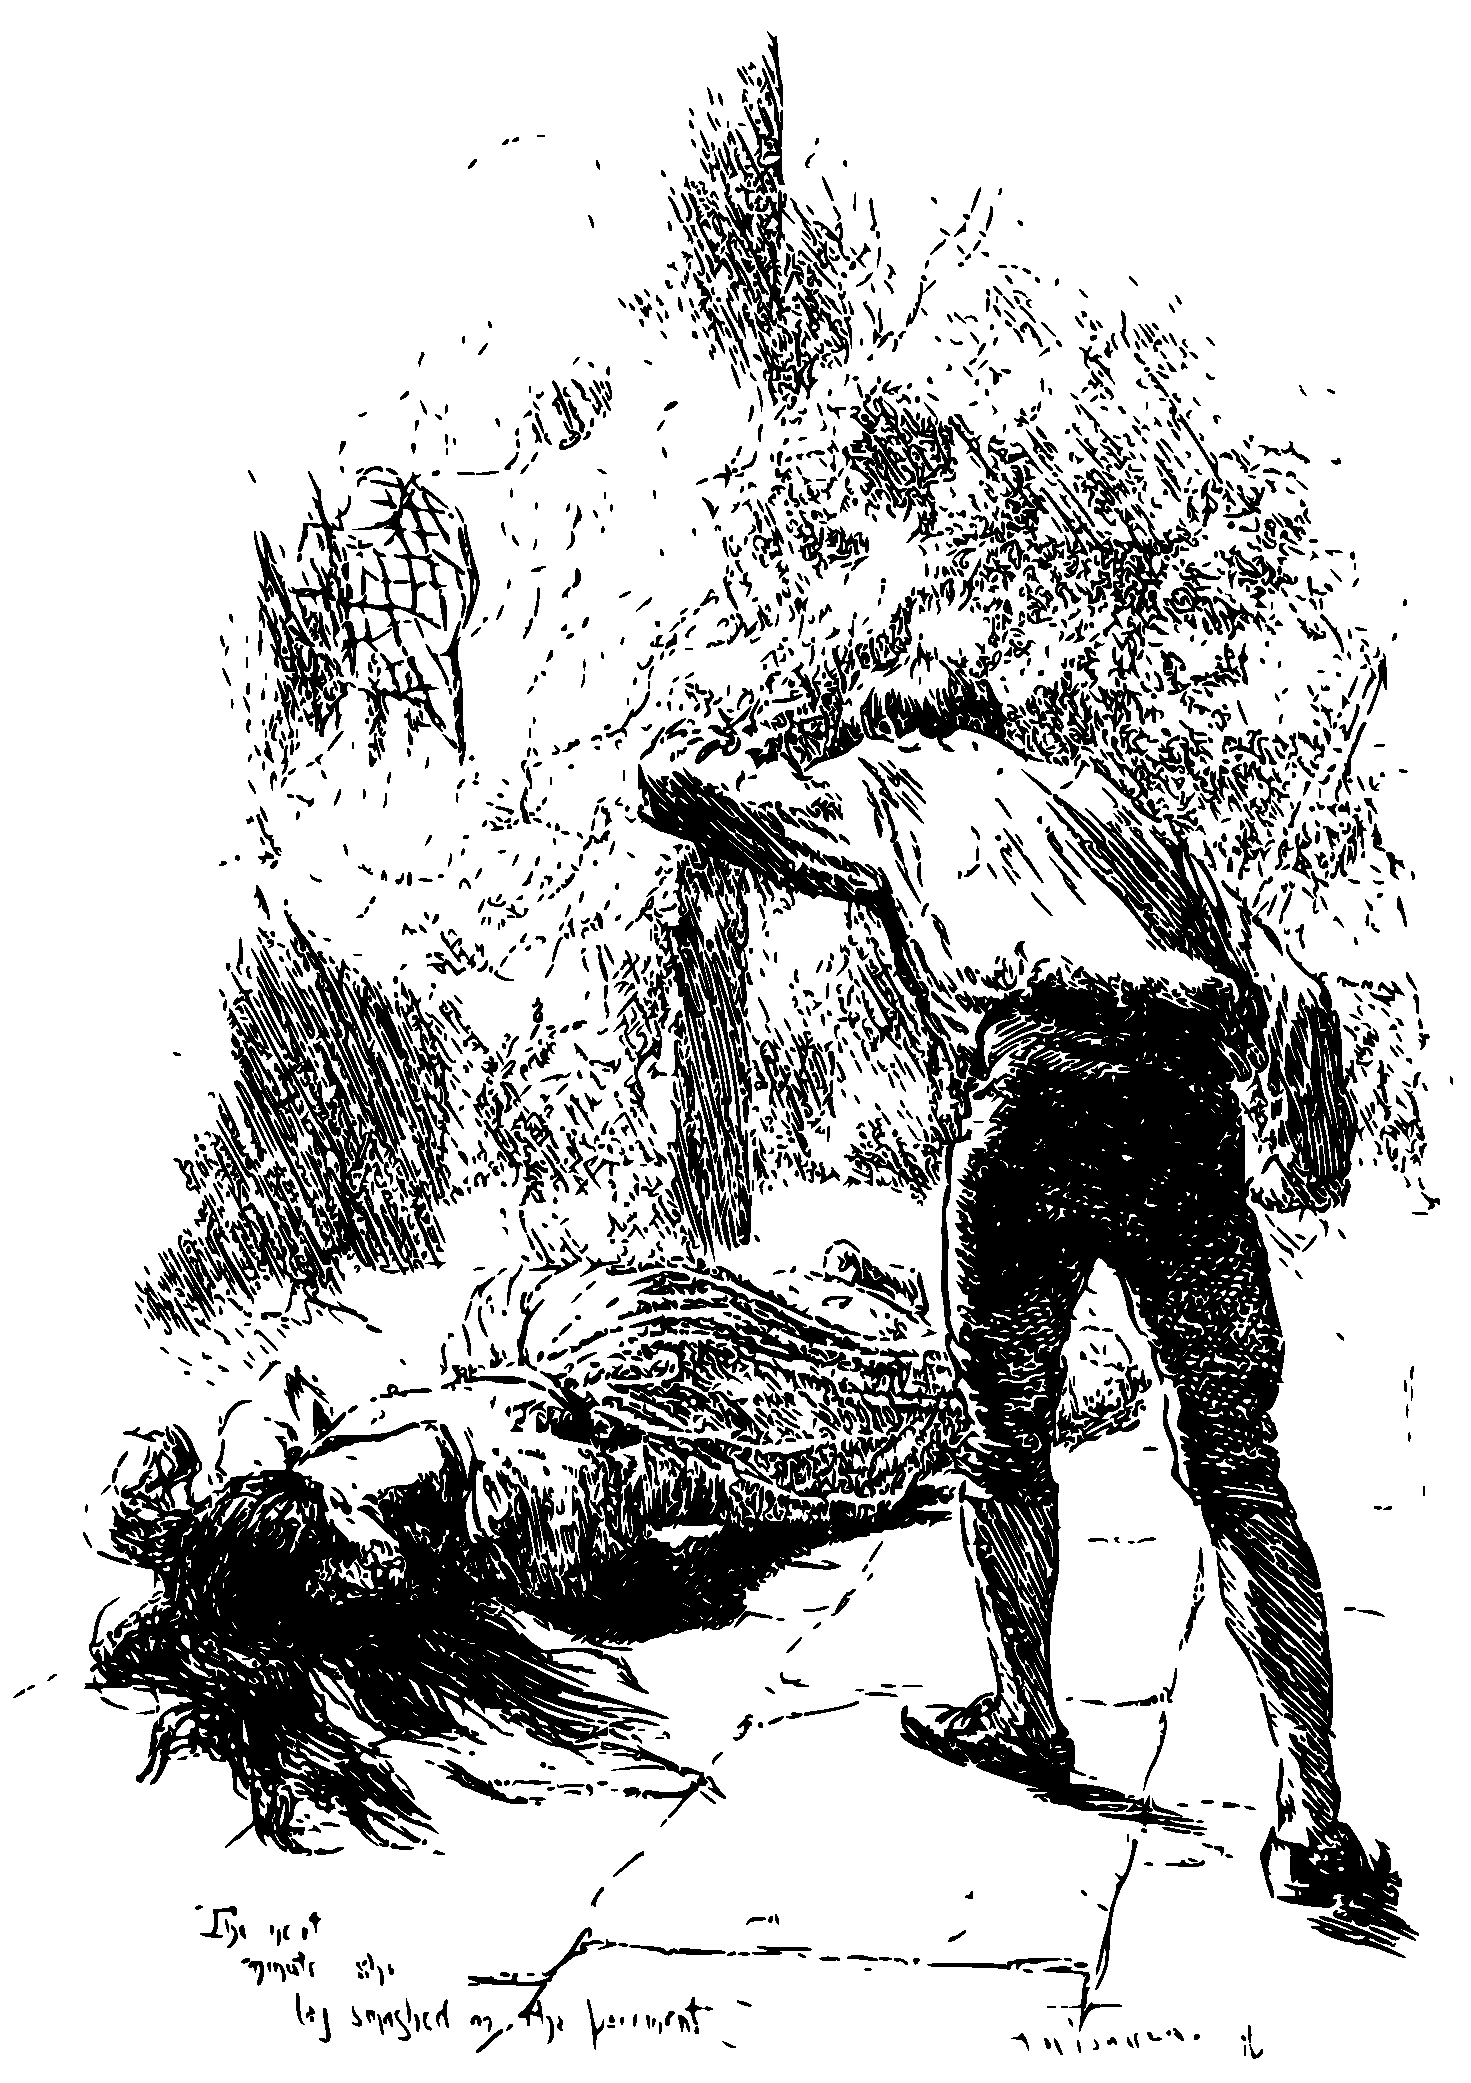
\includegraphics[width=\linewidth]{images/p413b.pdf}
	\end{sidecaption}
\end{figure}

\enquote{Dead?}

\enquote{Dead! Ay, dead as the stones on which her brains and blood
were scattered.}

\enquote{Good God!}

\enquote{You may well say so, ma'am: it was frightful!}

He shuddered.

\enquote{And afterwards?} I urged.

\enquote{Well, ma'am, afterwards the house was burnt to the ground:
there are only some bits of walls standing now.}

\enquote{Were any other lives lost?}

\enquote{No---perhaps it would have been better if there had.}

\enquote{What do you mean?}

\enquote{Poor \Mr{} Edward!} he ejaculated, \enquote{I little thought ever
to have seen it! Some say it was a just judgment on him for keeping his
first marriage secret, and wanting to take another wife while he had one
living: but I pity him, for my part.}

\enquote{You said he was alive?} I exclaimed.

\enquote{Yes, yes: he is alive; but many think he had better be dead.}

\enquote{Why? How?} My blood was again running cold. \enquote{Where
is he?} I demanded. \enquote{Is he in England?}

\enquote{Ay---ay---he's in England; he can't get out of England, I
fancy---he's a fixture now.}

What agony was this! And the man seemed resolved to protract it.

\enquote{He is stone-blind,} he said at last. \enquote{Yes, he is
stone-blind, is \Mr{} Edward.}

I had dreaded worse. I had dreaded he was mad. I summoned strength to
ask what had caused this calamity.

\enquote{It was all his own courage, and a body may say, his kindness,
in a way, ma'am: he wouldn't leave the house till every one else was out
before him. As he came down the great staircase at last, after \Mrs{}
 Rochester had flung herself from the battlements, there was a great
crash---all fell. He was taken out from under the ruins, alive, but
sadly hurt: a beam had fallen in such a way as to protect him partly;
but one eye was knocked out, and one hand so crushed that \Mr{} Carter,
the surgeon, had to amputate it directly. The other eye inflamed: he
lost the sight of that also. He is now helpless, indeed---blind and a
cripple.}

\enquote{Where is he? Where does he now live?}

\enquote{At Ferndean, a manor-house on a farm he has, about thirty miles
off: quite a desolate spot.}

\enquote{Who is with him?}

\enquote{Old John and his wife: he would have none else. He is quite
broken down, they say.}

\enquote{Have you any sort of conveyance?}

\enquote{We have a chaise, ma'am, a very handsome chaise.}

\enquote{Let it be got ready instantly; and if your post-boy can drive
me to Ferndean before dark this day, I'll pay both you and him twice the
hire you usually demand.}
